\section{Empirical evaluation}

We first present our experimental setup and implementation details in Sec.~\ref{sec:exp_setup}, before ablating various components of our model in Sec.~\ref{sec:exp_ablation}. We then present state-of-the-art results on five datasets in Sec.~\ref{sec:exp_sota_comparison}.

\subsection{Experimental Setup}\label{sec:exp_setup}

\paragraph{Network architecture and training}
Our backbone architecture follows that of ViT~\cite{dosovitskiy_iclr_2021} and BERT~\cite{devlin_naacl_2019}. We consider ViT-Base (ViT-B, $L$=$12$, $N_H$=$12$, $d$=$768$), ViT-Large (ViT-L, $L$=$24$, $N_H$=$16$, $d$=$1024$), and ViT-Huge (ViT-H, $L$=$32$, $N_H$=$16$, $d$=$1280$), where $L$ is the number of transformer layers, each with a self-attention block of $N_H$ heads and hidden dimension $d$. 
We also apply the same naming scheme to our models (e.g., ViViT-B/16x2 denotes a ViT-Base backbone with a tubelet size of $h \times w \times t = 16 \times  16 \times  2$). In all experiments, the tubelet height and width are equal. 
Note that smaller tubelet sizes correspond to more tokens at the input, and thus more computation.

We train our models using synchronous SGD and momentum, a cosine learning rate schedule and TPU-v3 accelerators. %
We initialise our models from a ViT image model trained either on ImageNet-21K~\cite{deng_cvpr_2009} (unless otherwise specified) or the larger JFT~\cite{sun_iccv_2017} dataset.
We implement our method using the Scenic library~\cite{dehghani2021scenic} and have released our code and models.

\paragraph{Datasets}

We evaluate the performance of our proposed models on a diverse set of video classification datasets:

\emph{Kinetics}~\cite{kay_arxiv_2017} consists of 10-second videos sampled at 25fps from YouTube.
We evaluate on both Kinetics 400 and 600, containing 400 and 600 classes respectively.
As these are dynamic datasets (videos may be removed from YouTube), we note our dataset sizes are approximately 267 000 and 446 000 respectively.

\emph{Epic Kitchens-100} consists of egocentric videos capturing daily kitchen activities spanning 100 hours and 90 000 clips~\cite{damen_arxiv_2020}.
We report results following the standard ``action recognition'' protocol.
Here, each video is labelled with a ``verb'' and a ``noun'' and we therefore predict both categories using a single network with two ``heads''. The top-scoring verb and action pair predicted by the network form an ``action'', and action accuracy is the primary metric.

\emph{Moments in Time}~\cite{monfort_pami_2019} consists of 800 000,  3-second YouTube clips that capture the gist of a dynamic scene involving animals, objects, people, or natural phenomena. 

\emph{Something-Something v2} (SSv2)~\cite{goyal_iccv_2017} contains 220 000 videos, with durations ranging from 2 to 6 seconds.
In contrast to the other datasets, the objects and backgrounds in the videos are consistent across different action classes, and this dataset thus places more emphasis on a model's ability to recognise fine-grained motion cues.

\begin{table}[t]
	\centering
	\caption{Comparison of input encoding methods using ViViT-B and spatio-temporal attention on Kinetics. 
	Further details in text.
	}
	\vspace{.1em}
	\begin{tabular}{lc}
		\toprule
		& Top-1 accuracy \\ \midrule
		Uniform frame sampling 		& 78.5          \\  %
		\midrule
		\textit{Tubelet embedding} \\
		Random initialisation~\cite{glorot_aistats_2010}  			& 73.2          \\ %
		Filter inflation~\cite{carreira_cvpr_2017}      				  & 77.6          \\ %
		Central frame          				& 79.2          \\ %
		\bottomrule
	\end{tabular}
	\vspace{-4mm}
	\label{tab:ablation_input_encoding}
\end{table}




\paragraph{Inference}
The input to our network is a video clip of 32 frames using a stride of 2, unless otherwise mentioned, similar to~\cite{feichtenhofer_iccv_2019, feichtenhofer_cvpr_2020}.
Following common practice, at inference time, we process multiple views of a longer video and average per-view logits to obtain the final result.
Unless otherwise specified, we use a total of 4 views per video (as this is sufficient to ``see'' the entire video clip across the various datasets), and ablate these and other design choices next.


\subsection{Ablation study}
\label{sec:exp_ablation}

\paragraph{Input encoding}
We first consider the effect of different input encoding methods (Sec.~\ref{sec:method_input_encoding}) using our unfactorised model (Model 1) and ViViT-B on Kinetics 400. 
As we pass 32-frame inputs to the network, sampling 8 frames and extracting tubelets of length $t = 4$ correspond to the same number of tokens in both cases.
Table~\ref{tab:ablation_input_encoding} shows that tubelet embedding initialised using the ``central frame'' method (Eq.~\ref{eq:central_frame_init}) performs well, outperforming the commonly-used ``filter inflation'' initialisation method~\cite{carreira_cvpr_2017, feichtenhofer_neurips_2016} by 1.6\%, and ``uniform frame sampling'' by 0.7\%.
We therefore use this encoding method for all subsequent experiments.


\begin{table}[tb]
	\centering
	\caption{Comparison of model architectures using ViViT-B as the backbone, and tubelet size of $16 \times 2$.
		We report Top-1 accuracy on Kinetics 400 (K400) and action accuracy on Epic Kitchens (EK).
		Runtime is during inference on a TPU-v3.
	}
	\scalebox{0.72}{
		\begin{tabular}{l M{0.09\linewidth} M{0.09\linewidth} M{0.13\linewidth} M{0.13\linewidth} M{0.13\linewidth}}
			\toprule
			& K400 & EK & FLOPs ($\times10^{9}$) & Params ($\times10^{6}$) & Runtime (ms) \\ \midrule
			Model 1: Spatio-temporal           			 &  80.0            &    43.1            &   455.2  & 88.9  &  58.9       \\			%
			Model 2: Fact. encoder        			&  78.8            &     43.7           &   284.4    & 115.1 &  17.4              \\   %
			Model 3: Fact. self-attention 		 &   77.4     &     39.1           &    372.3         &  117.3 &  31.7          \\  %
			Model 4: Fact. dot product    		 &   76.3       &       39.5         &    277.1    &  88.9 &  22.9         \\  %
			\midrule
			Model 2: Ave. pool baseline    & 75.8 &     38.8 	& 283.9 &	86.7 &  17.3  \\ %
			\bottomrule
		\end{tabular}
		\vspace{-5mm}
		\label{tab:ablation_model_variants}
	}
\end{table}




\begin{table}[tb]
	\centering
	\caption{The effect of varying the number of temporal transformers, $L_t$, in the Factorised encoder model (Model 2).
		We report the Top-1 accuracy on Kinetics 400.
		Note that $L_t = 0$ corresponds to the ``average pooling baseline''.
	}
	\begin{tabular}{lccccc}
	\toprule
	 $L_t$    			& 0 & 1 & 4 & 8 & 12 \\ \midrule
	 Top-1		& 75.8  & 78.6   & 78.8  & 78.8  & 78.9   \\ \bottomrule
	\end{tabular}
	\label{tab:ablation_temporal_transformers}
	\vspace{-\baselineskip}
\end{table}

\paragraph{Model variants}
We compare our proposed model variants (Sec.~\ref{sec:method_video_models}) across the Kinetics 400 and Epic Kitchens datasets, both in terms of accuracy and efficiency, in Tab.~\ref{tab:ablation_model_variants}.
In all cases, we use the ``Base'' backbone and tubelet size of $16 \times 2$.
Model 2 (``Factorised Encoder'') has an additional hyperparameter, the number of temporal transformers, $L_t$.
We set $L_t = 4$ for all experiments and show in Tab.~\ref{tab:ablation_temporal_transformers} that the model is not sensitive to this choice.

The unfactorised model (Model 1) performs the best on Kinetics 400.
However, it can also overfit on smaller datasets such as Epic Kitchens, where we find our ``Factorised Encoder'' (Model 2) to perform the best.
We also consider an additional baseline (last row), based on Model 2, where we do not use any temporal transformer, and simply average pool the frame-level representations from the spatial encoder before classifying.
This average pooling baseline performs the worst, and has a larger accuracy drop on Epic Kitchens, suggesting that this dataset requires more detailed modelling of temporal relations.

As described in Sec.~\ref{sec:method_video_models}, all factorised variants of our model use significantly fewer FLOPs than the unfactorised Model 1, as the attention is computed separately over spatial- and temporal-dimensions.
Model 4 adds no additional parameters to the unfactorised Model 1, and uses the least compute.
The temporal transformer encoder in Model 2 operates on only $n_t$ tokens, which is why there is a barely a change in compute and runtime over the average pooling baseline, even though it improves the accuracy substantially (3\% on Kinetics and 4.9\% on Epic Kitchens).
Finally, Model 3 requires more compute and parameters than the other factorised models, as its additional self-attention block means that it performs another query-, key-, value- and output-projection in each transformer layer~\cite{vaswani_neurips_2017}.


\begin{table}[t]
	\centering
	\caption{
		The effect of progressively adding regularisation (each row includes all methods above it) on Top-1 action accuracy on Epic Kitchens.
		We use a Factorised encoder model with tubelet size $16 \times 2$.
	}
	\small{  %
		\begin{tabular}{lcc}
			\toprule 
			& Top-1 accuracy  \\ 
			\midrule
			Random crop, flip, colour jitter           &      38.4   		\\   %
			+ Kinetics 400 initialisation 				 &      39.6  		\\  %
			+ Stochastic depth~\cite{huang_stochasticdepth_eccv_2016}       				 &      40.2 			\\  %
			+ Random augment~\cite{cubuk_arxiv_2019}             				&      41.1 	 \\   %
			+ Label smoothing~\cite{szegedy_cvpr_2016}             				  &      43.1      \\   %
			+ Mixup~\cite{zhang_mixup_iclr_2018}                       	 	  				&      43.7 	   \\   %
			\bottomrule
		\end{tabular}
	}
	\label{tab:regularisation_epic_kitchens}
	\vspace{-\baselineskip}
\end{table}



\begin{figure}[t]
	\centering
	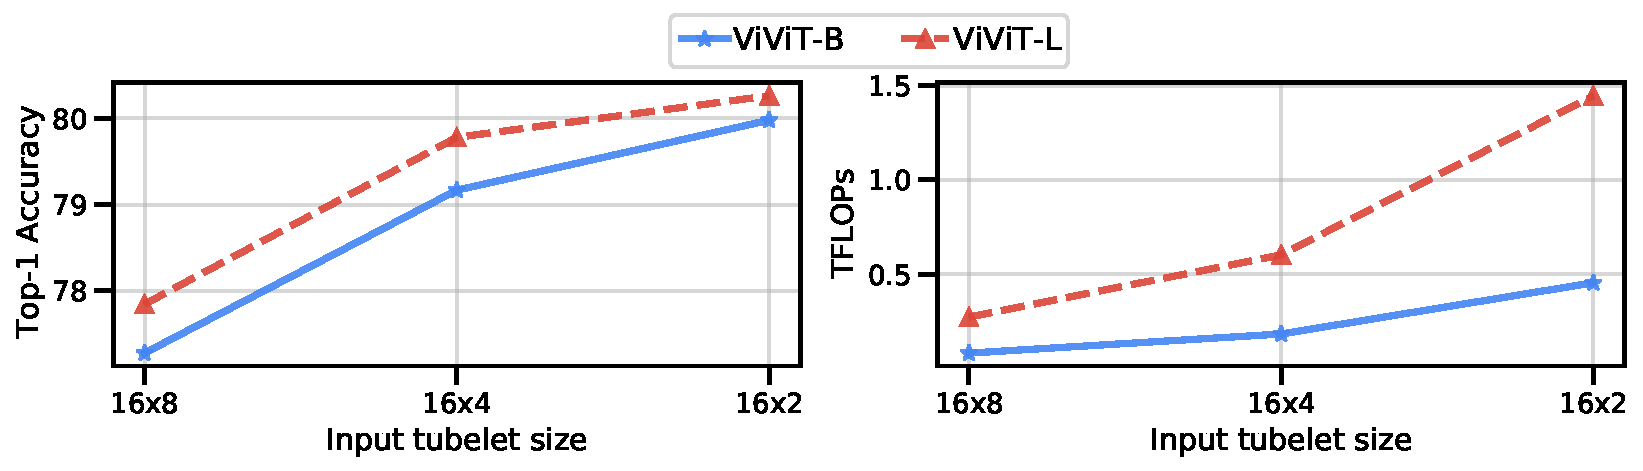
\includegraphics[width=\linewidth]{figures/ablation/patch_size_backbone}
	\footnotesize{
    	\begin{tabularx}{\linewidth}{YY}
    	    (a) Accuracy   &  (b) Compute
    	\end{tabularx}
	}
	\caption{The effect of the backbone architecture on (a) accuracy and (b) computation %
	on Kinetics 400, for the spatio-temporal attention model (Model 1).
	}
	\label{fig:ablation_backbone}
	\vspace{-0.5\baselineskip}
\end{figure}

\begin{figure}[t]
	\centering
	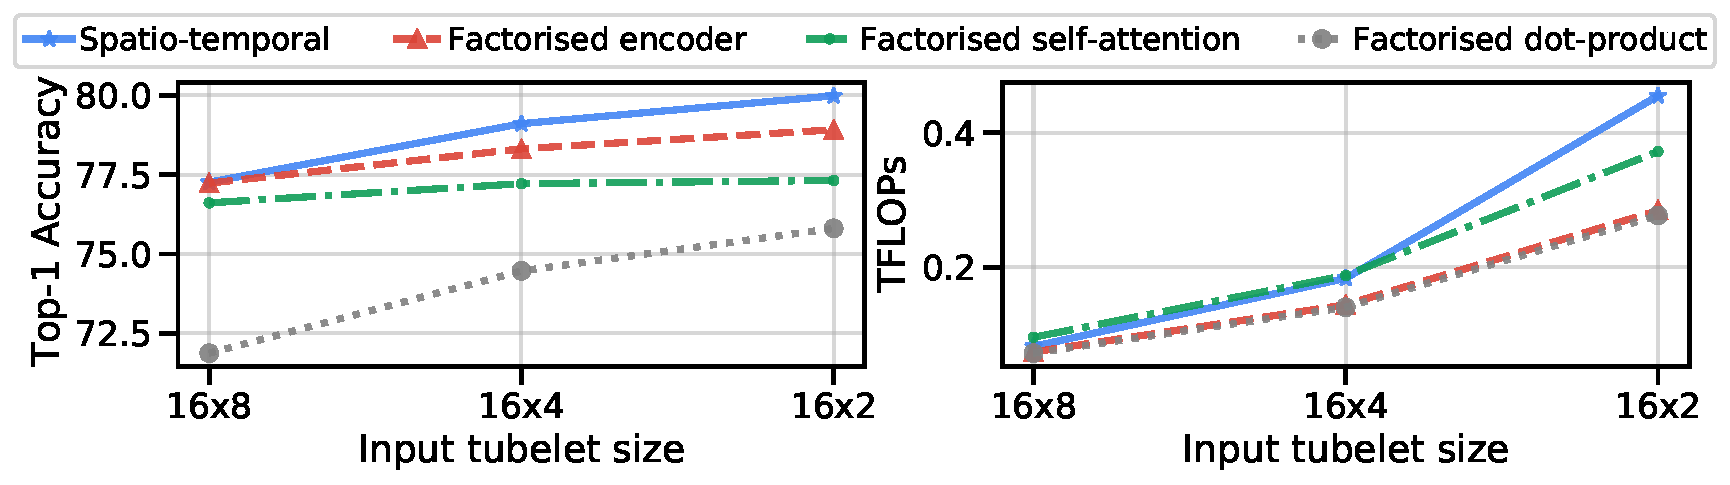
\includegraphics[width=\linewidth]{figures/ablation/patch_size_variants}
	\\
	\footnotesize{
    	\begin{tabularx}{\linewidth}{YY}
    	    (a) Accuracy   &  (b) Compute
    	\end{tabularx}
	}
 	\vspace{-0.5\baselineskip}
	\caption{The effect of varying the number of temporal tokens on (a) accuracy and (b) computation %
	on Kinetics 400, for different variants of our model with a ViViT-B backbone.
	}
	\label{fig:ablation_temporal_tokens}
	\vspace{-\baselineskip}
\end{figure}


\paragraph{Model regularisation}
Pure-transformer architectures such as ViT~\cite{dosovitskiy_iclr_2021} are known to require large training datasets, and we observed overfitting on smaller datasets like Epic Kitchens and SSv2, even when using an ImageNet pretrained model.
In order to effectively train our models on such datasets, we employed several regularisation strategies that we ablate using our ``Factorised encoder'' model in Tab.~\ref{tab:regularisation_epic_kitchens}.
We note that these regularisers were originally proposed for training CNNs, and that~\cite{touvron_arxiv_2020} have recently explored them for training ViT for image classification.

Each row of Tab.~\ref{tab:regularisation_epic_kitchens} includes all the methods from the rows above it, and we observe progressive improvements from adding each regulariser.
Overall, we obtain a substantial overall improvement of 5.3\% on Epic Kitchens. %
We also achieve a similar improvement of 5\% %
on SSv2 by using all the regularisation in Tab.~\ref{tab:regularisation_epic_kitchens}.
Note that the Kinetics-pretrained models that we initialise from are from Tab.~\ref{tab:ablation_model_variants}, and that all Epic Kitchens models in Tab.~\ref{tab:ablation_model_variants} were trained with all the regularisers in Tab.~\ref{tab:regularisation_epic_kitchens}.
For larger datasets like Kinetics and Moments in Time, we do not use these additional regularisers (we use only the first row of Tab.~\ref{tab:regularisation_epic_kitchens}), as we obtain state-of-the-art results without them.
The appendix contains hyperparameter values and additional details for all regularisers.


\paragraph{Varying the backbone}
Figure~\ref{fig:ablation_backbone} compares the ViViT-B and ViViT-L backbones for the unfactorised spatio-temporal model. We observe consistent improvements in accuracy as the backbone capacity increases. As expected, the compute also grows as a function of the backbone size.

\begin{table}[t]
	\centering
	\caption{The effect of spatial resolution on the performance of ViViT-L/16x2 and spatio-temporal attention on Kinetics 400.}
	\vspace{0.1em}
	\small{
	\begin{tabular}{lccc}
		\toprule
		Crop size & 224         & 288         & 320        \\ \midrule
		Accuracy &   80.3          &  80.7            &   81.0         \\   %
		GFLOPs    &     1446        &   2919          &   3992         \\
		Runtime  &     58.9        &      147.6       &    238.8       \\
		\bottomrule
	\end{tabular}
	\vspace{-0.5\baselineskip}
	\label{tab:ablation_spatial_resolution}
	}
\end{table}



\paragraph{Varying the number of tokens}
We first analyse the performance as a function of the number of tokens along the temporal dimension %
in Fig.~\ref{fig:ablation_temporal_tokens}. 
We observe that using smaller input tubelet sizes (and therefore more tokens) leads to consistent accuracy improvements across all of our model architectures.
At the same time, computation in terms of FLOPs increases accordingly, and the unfactorised model (Model 1) is impacted the most.

We then vary the number of tokens fed into the model by increasing the spatial crop-size from the default of 224 to 320 in Tab.~\ref{tab:ablation_spatial_resolution}.
As expected, there is a consistent increase in both accuracy and computation. We note that when comparing to prior work we consistently obtain state-of-the-art results (Sec.~\ref{sec:exp_sota_comparison}) using a spatial resolution of 224, but we also highlight that further improvements can be obtained at higher spatial resolutions.


\begin{table*}[tb]
	\caption{Comparisons to state-of-the-art across multiple datasets. For ``views'', $x \times y$ denotes $x$ temporal crops and $y$ spatial crops.
	We report the TFLOPs to process all spatio-temporal views.
	``FE'' denotes our Factorised Encoder model.
	}
	\vspace{0.2\baselineskip}
	\begin{subtable}[t]{.40\linewidth}
		\centering
		\caption{Kinetics 400}
    	\setlength{\tabcolsep}{4pt} %
		\renewcommand*{\arraystretch}{1.11}  %
		
		\vspace{-0.3\baselineskip}
		\scriptsize{
			\begin{tabular}{lcccc}
				\toprule
				Method 																			 & Top 1                & Top 5         & Views 	& TFLOPs \\
				\midrule
				blVNet~\cite{fan_blvnet_neurips_2019}							  & 73.5 				  & 91.2  & --  & --\\ 
				STM~\cite{jiang_stm_iccv_2019}										& 73.7 					& 91.6	& -- & -- \\
				TEA~\cite{li_tea_cvpr_2020}												& 76.1					& 92.5 & $10 \times 3$ & 2.10 \\  %
				TSM-ResNeXt-101~\cite{lin_tsm_cvpr_2019}						  & 76.3				 & -- &  -- & -- \\
				I3D NL~\cite{wang_cvpr_2018}										 & 77.7                  & 93.3         		 &  $10 \times 3$ & 10.77     \\  %
				CorrNet-101~\cite{wang_corrnet_cvpr_2020}					  & 79.2				 & --			 		 & $10 \times 3$	& 6.72	 \\  %
				ip-CSN-152~\cite{tran_iccv_2019}									&  79.2					& 93.8				& $10 \times 3$	& 3.27	 \\  %
				LGD-3D R101~\cite{qiu_lgd_cvpr_2019}							&  79.4				    & 94.4			 		&  --	& --					\\  
				SlowFast R101-NL~\cite{feichtenhofer_iccv_2019}       		&  79.8                 &  93.9                   & $10 \times 3$    & 7.02   \\  %
				X3D-XXL~\cite{feichtenhofer_cvpr_2020}      					&  80.4					&  94.6			  		& $10 \times 3$   & 5.82   \\
				TimeSformer-L~\cite{bertasius_arxiv_2021}					  	& 80.7				& \textbf{94.7}					& $1 \times 3$ & 7.14 \\
				ViViT-L/16x2 FE 														  	 &  80.6 				& 92.7 & $1 \times 1$   & 3.98 \\  %
				ViViT-L/16x2 FE 															& \textbf{81.7} 	&  93.8  & $1 \times 3$ &  11.94 \\  %
				\midrule
				\multicolumn{4}{l}{\textit{Methods with large-scale pretraining}}                                \\ 
				ip-CSN-152~\cite{tran_iccv_2019} (IG~\cite{mahajan_eccv_2018}) 			  &  82.5					& 95.3			&  $10 \times 3$ & 3.27	  \\
				ViViT-L/16x2 FE (JFT) 														& 83.5 	&  94.3   & $1 \times 3$ &  11.94 \\  %
				ViViT-H/14x2 (JFT) 														&  \textbf{84.9} &  \textbf{95.8} 	& $4 \times 3$ & 47.77 \\  %
				\bottomrule
			\end{tabular}
		}
		\label{tab:sota_kinetics400}
	\end{subtable}
  	\hfill
  	\begin{subtable}[t]{.28\linewidth}
		\centering
  		\caption{Kinetics 600}
  		\setlength{\tabcolsep}{4pt} %
		\vspace{-0.3\baselineskip}
  		\scriptsize{
	  		\begin{tabular}{lcc}
	  			\toprule
	  			Method 																			 & Top 1                & Top 5      \\ %
	  			\midrule
	  			AttentionNAS~\cite{wang_nas_eccv_2020}						  &  79.8				   & 94.4  \\ %
	  			LGD-3D R101~\cite{qiu_lgd_cvpr_2019}							&  81.5				    & 95.6	\\ %
	  			SlowFast R101-NL~\cite{feichtenhofer_iccv_2019}       		&  81.8                     &  95.1   \\ %
	  			X3D-XL~\cite{feichtenhofer_cvpr_2020}      						 &  81.9					&  95.5		\\ %
	  			TimeSformer-L~\cite{bertasius_arxiv_2021}					  & 82.2				& \textbf{95.6}		\\ %
	  			ViViT-L/16x2 FE 														  	 &  \textbf{82.9} 	& 94.6  \\  %
	  			%
	  			%
	  			\midrule
	  			ViViT-L/16x2 FE (JFT) 													 & 84.3 & 94.9 \\ %
	  			%
	  			ViViT-H/14x2 (JFT) 													& \textbf{85.8} & \textbf{96.5} \\ %
	  			\bottomrule
	  		\end{tabular}
	  		\label{tab:sota_kinetics600}
  		}
  		\vspace{0.35\baselineskip} %
  		\centering
  		\caption{Moments in Time}
  		\vspace{-0.3\baselineskip}
  		\setlength{\tabcolsep}{6pt} %
  		\scriptsize{
  			\begin{tabular}{lcc}
  				\toprule
  				& Top 1 & Top 5 \\ 
  				\midrule
  				TSN~\cite{wang_tsn_eccv_2016}				& 25.3		 &  50.1	\\
  				TRN~\cite{zhou_trn_eccv_2018}				 & 28.3		 &  53.4	 \\
  				I3D~\cite{carreira_cvpr_2017}					& 29.5		&  56.1		\\
  				blVNet~\cite{fan_blvnet_neurips_2019}	 &  31.4	 &  59.3 	 \\
  				AssembleNet-101~\cite{ryoo_iclr_2020} 	&  34.3     &  62.7     \\
  				\midrule
  				ViViT-L/16x2 FE 	& \textbf{38.5} & \textbf{64.1} \\  %
  				\bottomrule
  			\end{tabular}
  			\label{tab:sota_moments_in_time}
  		}
  	\end{subtable}
  	\hfill
  	\begin{subtable}[t]{.28\linewidth}
  		\caption{Epic Kitchens 100 Top 1 accuracy}
  		\setlength{\tabcolsep}{4pt} %
  		\vspace{-0.3\baselineskip}
		\scriptsize{
			\begin{tabular}{lccc}
				\toprule
				Method 													 & Action & Verb  & Noun  \\
				\midrule
				TSN~\cite{wang_tsn_eccv_2016}		 		&  33.2 & 60.2 & 46.0  \\
				TRN~\cite{zhou_trn_eccv_2018} 				& 35.3 & 65.9 & 45.4   \\
				TBN~\cite{kazakos_iccv_2019}				 & 36.7 & 66.0 & 47.2    \\
				TSM~\cite{lin_tsm_cvpr_2019} 				 & 38.3 & \textbf{67.9} & 49.0  \\
				SlowFast~\cite{feichtenhofer_iccv_2019}  & 38.5 & 65.6 & 50.0  \\
				\midrule
				ViViT-L/16x2 FE & \textbf{44.0} & 66.4 & \textbf{56.8} \\ %
				\bottomrule
			\end{tabular}
		}
		\label{tab:sota_epic_kitchens}
		\vspace{0.4\baselineskip}
		\centering
		\caption{Something-Something v2}
		\setlength{\tabcolsep}{6pt} %
		\scriptsize{
			\begin{tabular}{lcc}
				\toprule
				Method 												  & Top 1                & Top 5   \\
				\midrule
				TRN~\cite{zhou_trn_eccv_2018}										& 48.8 & 77.6 \\
				SlowFast~\cite{feichtenhofer_cvpr_2020,wu_multigrid_cvpr_2020}		& 61.7 & --    \\
				TimeSformer-HR~\cite{bertasius_arxiv_2021}					& 62.5 & -- \\
				TSM~\cite{lin_tsm_cvpr_2019}    		   							& 63.4 & 88.5 \\
				STM~\cite{jiang_stm_iccv_2019}				   						& 64.2 & 89.8 \\
				TEA~\cite{li_tea_cvpr_2020}						   					& 65.1 & -- \\
				blVNet~\cite{fan_blvnet_neurips_2019}  		 						& 65.2  & \textbf{90.3} \\
				\midrule
				ViVIT-L/16x2 FE		& \textbf{65.9}  & 89.9 \\ %
				\bottomrule
			\end{tabular}
			\label{tab:sota_ssv2}
		}
	\end{subtable}
	\vspace{-\baselineskip}
\end{table*}

\begin{figure}[tb]
	\centering
	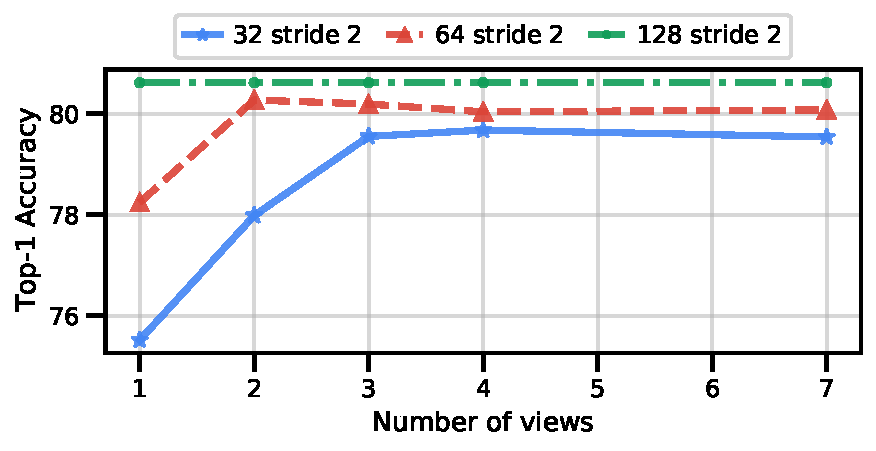
\includegraphics[width=0.95\linewidth]{figures/ablation/views_accuracy_frames.pdf}
	\caption{
		The effect of varying the number of frames input to the network and increasing the number of tokens proportionally.
		We use ViViT-L/16x2 Factorised Encoder on Kinetics 400.
		A Kinetics video contains 250 frames (10 seconds sampled at 25 fps) and the accuracy for each model saturates once the number of equidistant temporal views is sufficient to ``see'' the whole video clip.
		Observe how models processing more frames (and thus more tokens) achieve higher single- and multi-view accuracy.
	}
	\label{fig:ablation_num_frames}
	\vspace{-\baselineskip}
\end{figure}
\paragraph{Varying the number of input frames}




In our experiments so far, we have kept the number of input frames fixed at 32.
We now increase the number of frames input to the model, thereby increasing the number of tokens proportionally.

Figure~\ref{fig:ablation_num_frames} shows that as we increase the number of frames input to the network, the accuracy from processing a single view increases, since the network incorporates longer temporal context.
However, common practice on datasets such as Kinetics~\cite{feichtenhofer_iccv_2019, wang_cvpr_2018, li_tea_cvpr_2020} is to average results over multiple, shorter ``views'' of the same video clip.
Figure~\ref{fig:ablation_num_frames} also shows that the accuracy saturates once the number of views is sufficient to cover the whole video.
As a Kinetics video consists of 250 frames, and we sample frames with a stride of 2, our model which processes 128 frames requires just a single view to ``see'' the whole video and achieve its maximum accuarcy.

Note that we used  ViViT-L/16x2 Factorised Encoder (Model 2) here.
As this model is more efficient it can process more tokens, compared to the unfactorised Model 1 which runs out of memory after 48 frames using tubelet length $t = 2$ and a ``Large'' backbone.
Models processing more frames (and thus more tokens) consistently achieve higher single- and multi-view accuracy, in line with our observations in previous experiments (Tab.~\ref{tab:ablation_spatial_resolution}, Fig.~\ref{fig:ablation_temporal_tokens}).
Moroever, observe that by processing more frames (and thus more tokens) with Model 2, we are able to achieve higher accuracy than Model 1 (with fewer total FLOPs as well).

Finally, we observed that for Model 2, the number of FLOPs effectively increases linearly with the number of input frames as the overall computation is dominated by the initial Spatial Transformer.
As a result, the total number of FLOPs for the number of temporal views required to achieve maximum accuracy is constant across the models.
In other words, ViViT-L/16x2 FE with 32 frames requires 995.3 GFLOPs per view, and 4 views to saturate multi-view accuracy.
The 128-frame model requires 3980.4 GFLOPs but only a single view.
As shown by Fig.~\ref{fig:ablation_num_frames}, the latter model achieves the highest accuracy.





\subsection{Comparison to state-of-the-art}\label{sec:exp_sota_comparison}
Based on our ablation studies in the previous section, we compare to the current state-of-the-art using two of our model variants.
We primarily use our Factorised Encoder model (Model 2), as it can process more tokens than Model 1 to achieve higher accuracy.

\vspace{-0\baselineskip}
\paragraph{Kinetics}
Tables~\ref{tab:sota_kinetics400} and ~\ref{tab:sota_kinetics600} show that our spatio-temporal attention models outperform the state-of-the-art on Kinetics 400 and 600 respectively.
Following standard practice, we take 3 spatial crops (left, centre and right)~\cite{feichtenhofer_iccv_2019,feichtenhofer_cvpr_2020,tran_iccv_2019,wang_cvpr_2018} for each temporal view, and notably, we require significantly fewer views than previous CNN-based methods.


We surpass the previous CNN-based state-of-the-art using ViViT-L/16x2 Factorised Encoder (FE) pretrained on ImageNet, and also outperform~\cite{bertasius_arxiv_2021} who concurrently proposed a pure-transformer architecture.
Moreover, by initialising our backbones from models pretrained on the larger JFT dataset~\cite{sun_iccv_2017}, we obtain further improvements. Although these models are not directly comparable to previous work, we do also outperform~\cite{tran_iccv_2019} who pretrained on the large-scale, Instagram dataset~\cite{mahajan_eccv_2018}. Our best model uses a ViViT-H backbone pretrained on JFT and significantly advances the best reported results on Kinetics 400 and 600 to 84.9\% and 85.8\%, respectively.

\vspace{-0\baselineskip}
\paragraph{Moments in Time}
We surpass the state-of-the-art by a significant margin as shown in Tab.~\ref{tab:sota_moments_in_time}. 
We note that the videos in this dataset are diverse and contain significant label  noise, making this task challenging and leading to lower accuracies than on other datasets.

\vspace{-0\baselineskip}
\paragraph{Epic Kitchens 100}
Table~\ref{tab:sota_epic_kitchens} shows that our Factorised Encoder model outperforms previous methods by a significant margin. In addition, our model obtains substantial improvements for Top-1 accuracy of ``noun'' classes, and the only method which achieves higher ``verb'' accuracy used optical flow as an additional input modality~\cite{lin_tsm_cvpr_2019, price_arxiv_2019}. 
Furthermore, all variants of our model presented in Tab.~\ref{tab:ablation_model_variants} outperformed the existing state-of-the-art on  action accuracy.
We note that we use the same model to predict verbs and nouns using two separate ``heads'', and for simplicity, we do not use separate loss weights for each head. 

\paragraph{Something-Something v2 (SSv2)}

Finally, Tab.~\ref{tab:sota_ssv2} shows that we achieve state-of-the-art Top-1 accuracy with our Factorised encoder model (Model 2), albeit with a smaller margin compared to previous methods.
Notably, our Factorised encoder model significantly outperforms the concurrent TimeSformer~\cite{bertasius_arxiv_2021} method by 2.9\%, which also proposes a pure-transformer model, but does not consider our Factorised encoder variant or our additional regularisation.

SSv2 differs from other datasets in that the backgrounds and objects are quite similar across different classes, meaning that recognising fine-grained motion patterns is necessary to distinguish classes from each other.
Our results suggest that capturing these fine-grained motions is an area of improvement and future work for our model.
We also note an inverse correlation between the relative performance of previous methods on SSv2 (Tab.~\ref{tab:sota_ssv2}) and Kinetics~(Tab.~\ref{tab:sota_kinetics400})
suggesting that these two datasets evaluate complementary characteristics of a model.

